\documentclass[conference,compsoc]{IEEEtran}
% Some/most Computer Society conferences require the compsoc mode option,
% but others may want the standard conference format.
%
% If IEEEtran.cls has not been installed into the LaTeX system files,
% manually specify the path to it like:
% \documentclass[conference,compsoc]{../sty/IEEEtran}





% Some very useful LaTeX packages include:
% (uncomment the ones you want to load)


% *** MISC UTILITY PACKAGES ***
%
%\usepackage{ifpdf}
% Heiko Oberdiek's ifpdf.sty is very useful if you need conditional
% compilation based on whether the output is pdf or dvi.
% usage:
% \ifpdf
%   % pdf code
% \else
%   % dvi code
% \fi
% The latest version of ifpdf.sty can be obtained from:
% http://www.ctan.org/pkg/ifpdf
% Also, note that IEEEtran.cls V1.7 and later provides a builtin
% \ifCLASSINFOpdf conditional that works the same way.
% When switching from latex to pdflatex and vice-versa, the compiler may
% have to be run twice to clear warning/error messages.






% *** CITATION PACKAGES ***
%
\ifCLASSOPTIONcompsoc
  % IEEE Computer Society needs nocompress option
  % requires cite.sty v4.0 or later (November 2003)
  \usepackage[nocompress]{cite}
\else
  % normal IEEE
  \usepackage{cite}
\fi
% cite.sty was written by Donald Arseneau
% V1.6 and later of IEEEtran pre-defines the format of the cite.sty package
% \cite{} output to follow that of the IEEE. Loading the cite package will
% result in citation numbers being automatically sorted and properly
% "compressed/ranged". e.g., [1], [9], [2], [7], [5], [6] without using
% cite.sty will become [1], [2], [5]--[7], [9] using cite.sty. cite.sty's
% \cite will automatically add leading space, if needed. Use cite.sty's
% noadjust option (cite.sty V3.8 and later) if you want to turn this off
% such as if a citation ever needs to be enclosed in parenthesis.
% cite.sty is already installed on most LaTeX systems. Be sure and use
% version 5.0 (2009-03-20) and later if using hyperref.sty.
% The latest version can be obtained at:
% http://www.ctan.org/pkg/cite
% The documentation is contained in the cite.sty file itself.
%
% Note that some packages require special options to format as the Computer
% Society requires. In particular, Computer Society  papers do not use
% compressed citation ranges as is done in typical IEEE papers
% (e.g., [1]-[4]). Instead, they list every citation separately in order
% (e.g., [1], [2], [3], [4]). To get the latter we need to load the cite
% package with the nocompress option which is supported by cite.sty v4.0
% and later.





% *** GRAPHICS RELATED PACKAGES ***
%
\ifCLASSINFOpdf
  % \usepackage[pdftex]{graphicx}
  % declare the path(s) where your graphic files are
  % \graphicspath{{../pdf/}{../jpeg/}}
  % and their extensions so you won't have to specify these with
  % every instance of \includegraphics
  % \DeclareGraphicsExtensions{.pdf,.jpeg,.png}
\else
  % or other class option (dvipsone, dvipdf, if not using dvips). graphicx
  % will default to the driver specified in the system graphics.cfg if no
  % driver is specified.
  % \usepackage[dvips]{graphicx}
  % declare the path(s) where your graphic files are
  % \graphicspath{{../eps/}}
  % and their extensions so you won't have to specify these with
  % every instance of \includegraphics
  % \DeclareGraphicsExtensions{.eps}
\fi
% graphicx was written by David Carlisle and Sebastian Rahtz. It is
% required if you want graphics, photos, etc. graphicx.sty is already
% installed on most LaTeX systems. The latest version and documentation
% can be obtained at: 
% http://www.ctan.org/pkg/graphicx
% Another good source of documentation is "Using Imported Graphics in
% LaTeX2e" by Keith Reckdahl which can be found at:
% http://www.ctan.org/pkg/epslatex
%
% latex, and pdflatex in dvi mode, support graphics in encapsulated
% postscript (.eps) format. pdflatex in pdf mode supports graphics
% in .pdf, .jpeg, .png and .mps (metapost) formats. Users should ensure
% that all non-photo figures use a vector format (.eps, .pdf, .mps) and
% not a bitmapped formats (.jpeg, .png). The IEEE frowns on bitmapped formats
% which can result in "jaggedy"/blurry rendering of lines and letters as
% well as large increases in file sizes.
%
% You can find documentation about the pdfTeX application at:
% http://www.tug.org/applications/pdftex




% *** ALIGNMENT PACKAGES ***
%
%\usepackage{array}
% Frank Mittelbach's and David Carlisle's array.sty patches and improves
% the standard LaTeX2e array and tabular environments to provide better
% appearance and additional user controls. As the default LaTeX2e table
% generation code is lacking to the point of almost being broken with
% respect to the quality of the end results, all users are strongly
% advised to use an enhanced (at the very least that provided by array.sty)
% set of table tools. array.sty is already installed on most systems. The
% latest version and documentation can be obtained at:
% http://www.ctan.org/pkg/array


% IEEEtran contains the IEEEeqnarray family of commands that can be used to
% generate multiline equations as well as matrices, tables, etc., of high
% quality.




% *** SUBFIGURE PACKAGES ***
\ifCLASSOPTIONcompsoc
  \usepackage[caption=false,font=footnotesize,labelfont=sf,textfont=sf]{subfig}
\else
  \usepackage[caption=false,font=footnotesize]{subfig}
\fi
% subfig.sty, written by Steven Douglas Cochran, is the modern replacement
% for subfigure.sty, the latter of which is no longer maintained and is
% incompatible with some LaTeX packages including fixltx2e. However,
% subfig.sty requires and automatically loads Axel Sommerfeldt's caption.sty
% which will override IEEEtran.cls' handling of captions and this will result
% in non-IEEE style figure/table captions. To prevent this problem, be sure
% and invoke subfig.sty's "caption=false" package option (available since
% subfig.sty version 1.3, 2005/06/28) as this is will preserve IEEEtran.cls
% handling of captions.
% Note that the Computer Society format requires a sans serif font rather
% than the serif font used in traditional IEEE formatting and thus the need
% to invoke different subfig.sty package options depending on whether
% compsoc mode has been enabled.
%
% The latest version and documentation of subfig.sty can be obtained at:
% http://www.ctan.org/pkg/subfig




% *** FLOAT PACKAGES ***
%
%\usepackage{fixltx2e}
% fixltx2e, the successor to the earlier fix2col.sty, was written by
% Frank Mittelbach and David Carlisle. This package corrects a few problems
% in the LaTeX2e kernel, the most notable of which is that in current
% LaTeX2e releases, the ordering of single and double column floats is not
% guaranteed to be preserved. Thus, an unpatched LaTeX2e can allow a
% single column figure to be placed prior to an earlier double column
% figure.
% Be aware that LaTeX2e kernels dated 2015 and later have fixltx2e.sty's
% corrections already built into the system in which case a warning will
% be issued if an attempt is made to load fixltx2e.sty as it is no longer
% needed.
% The latest version and documentation can be found at:
% http://www.ctan.org/pkg/fixltx2e


%\usepackage{stfloats}
% stfloats.sty was written by Sigitas Tolusis. This package gives LaTeX2e
% the ability to do double column floats at the bottom of the page as well
% as the top. (e.g., "\begin{figure*}[!b]" is not normally possible in
% LaTeX2e). It also provides a command:
%\fnbelowfloat
% to enable the placement of footnotes below bottom floats (the standard
% LaTeX2e kernel puts them above bottom floats). This is an invasive package
% which rewrites many portions of the LaTeX2e float routines. It may not work
% with other packages that modify the LaTeX2e float routines. The latest
% version and documentation can be obtained at:
% http://www.ctan.org/pkg/stfloats
% Do not use the stfloats baselinefloat ability as the IEEE does not allow
% \baselineskip to stretch. Authors submitting work to the IEEE should note
% that the IEEE rarely uses double column equations and that authors should try
% to avoid such use. Do not be tempted to use the cuted.sty or midfloat.sty
% packages (also by Sigitas Tolusis) as the IEEE does not format its papers in
% such ways.
% Do not attempt to use stfloats with fixltx2e as they are incompatible.
% Instead, use Morten Hogholm'a dblfloatfix which combines the features
% of both fixltx2e and stfloats:
%
% \usepackage{dblfloatfix}
% The latest version can be found at:
% http://www.ctan.org/pkg/dblfloatfix




% *** PDF, URL AND HYPERLINK PACKAGES ***
%
\usepackage{url}
% url.sty was written by Donald Arseneau. It provides better support for
% handling and breaking URLs. url.sty is already installed on most LaTeX
% systems. The latest version and documentation can be obtained at:
% http://www.ctan.org/pkg/url
% Basically, \url{my_url_here}.




% *** Do not adjust lengths that control margins, column widths, etc. ***
% *** Do not use packages that alter fonts (such as pslatex).         ***
% There should be no need to do such things with IEEEtran.cls V1.6 and later.
% (Unless specifically asked to do so by the journal or conference you plan
% to submit to, of course. )


% correct bad hyphenation here
\hyphenation{op-tical net-works semi-conduc-tor}

\usepackage{amsfonts,amsmath,latexsym,amssymb}
\usepackage{algorithm,algpseudocode}
\usepackage{graphicx,xcolor}
\usepackage{hyperref,cleveref}
\usepackage{tikz}
\usetikzlibrary{3d}
\usepackage{pgfplots}
\usepackage{pgfplotstable}
\usepackage{etoolbox}
\usetikzlibrary{patterns}
% to include our macros
\usepackage{ourmacros}


\begin{document}
%
% paper title
% Titles are generally capitalized except for words such as a, an, and, as,
% at, but, by, for, in, nor, of, on, or, the, to and up, which are usually
% not capitalized unless they are the first or last word of the title.
% Linebreaks \\ can be used within to get better formatting as desired.
% Do not put math or special symbols in the title.
\title{Parallel Nonnegative CP Decomposition of Dense Tensors}


% author names and affiliations
% use a multiple column layout for up to three different
% affiliations
\author{\IEEEauthorblockN{Grey Ballard and Koby Hayashi}
\IEEEauthorblockA{Wake Forest University\\
Winston Salem NC 27109 \\
Email: \{ballard,hayashi\}@wfu.edu}
\and
\IEEEauthorblockN{Ramakrishnan Kannan}
\IEEEauthorblockA{Oak Ridge National Laboratory\\
Oak Ridge, TN 37830\\
Email: kannanr@ornl.gov}}

% for blind submission
\author{}

% conference papers do not typically use \thanks and this command
% is locked out in conference mode. If really needed, such as for
% the acknowledgment of grants, issue a \IEEEoverridecommandlockouts
% after \documentclass

% for over three affiliations, or if they all won't fit within the width
% of the page (and note that there is less available width in this regard for
% compsoc conferences compared to traditional conferences), use this
% alternative format:
% 
%\author{\IEEEauthorblockN{Michael Shell\IEEEauthorrefmark{1},
%Homer Simpson\IEEEauthorrefmark{2},
%James Kirk\IEEEauthorrefmark{3}, 
%Montgomery Scott\IEEEauthorrefmark{3} and
%Eldon Tyrell\IEEEauthorrefmark{4}}
%\IEEEauthorblockA{\IEEEauthorrefmark{1}School of Electrical and Computer Engineering\\
%Georgia Institute of Technology,
%Atlanta, Georgia 30332--0250\\ Email: see http://www.michaelshell.org/contact.html}
%\IEEEauthorblockA{\IEEEauthorrefmark{2}Twentieth Century Fox, Springfield, USA\\
%Email: homer@thesimpsons.com}
%\IEEEauthorblockA{\IEEEauthorrefmark{3}Starfleet Academy, San Francisco, California 96678-2391\\
%Telephone: (800) 555--1212, Fax: (888) 555--1212}
%\IEEEauthorblockA{\IEEEauthorrefmark{4}Tyrell Inc., 123 Replicant Street, Los Angeles, California 90210--4321}}




% use for special paper notices
%\IEEEspecialpapernotice{(Invited Paper)}




% make the title area
\maketitle

% As a general rule, do not put math, special symbols or citations
% in the abstract
%!TEX root = icpp18.tex

\begin{abstract}
Non-negative matrix factorization (NMF), the problem of finding two non-negative low-rank factors whose product approximates an input matrix, is a useful tool for many data mining and scientific applications such as topic modeling in text mining and blind source separation in microscopy.
In this paper, we focus on scaling algorithms for NMF to very large sparse datasets and massively parallel machines by employing effective algorithms, communication patterns, and partitioning schemes that leverage the sparsity of the input matrix.
In the case of machine learning workflow, the 
computations after SpMM must deal with dense matrices, as Sparse-Dense matrix multiplication will result in a dense matrix. 
Hence, the partitioning strategy considering only SpMM will result in a huge imbalance in the overall workflow especially on computations after SpMM and in this specific case of NMF on non-negative least squares computations. 
Towards this, we consider two previous works developed for related problems, one that uses a fine-grained partitioning strategy using a point-to-point communication pattern and on that uses a checkerboard partitioning strategy using a collective-based communication pattern.
We show that a combination of the previous approaches balances the demands of the various computations within NMF algorithms and achieves high efficiency and scalability. From the experiments, we could see that our proposed algorithm communicates atleast
4x less than the collective and achieves upto 100x speed up over the baseline FAUN on real world datasets. Our algorithm was experimented in two different super computing platforms and we could scale up to 32000 processors on Bluegene/Q.  

%We propose a fine-grain communication scheme that can utilize arbitrary partitions of the matrices. For a more scalable parallel NMF algorithm, we employ effective 2D and fine-grain hypergraph partitions. If hypergraph partitioning gets expensive for the purpose of the application, researchers can resort to the proposed uniform and random 2D partitioning NMF algorithms. But in the latter, memory growth of intermediate dense matrices is exorbitant -- a major bottleneck to run in lesser number of nodes. Toward this, we propose memory efficient blocking 2D matrix multiplication for sparse NMF. We compare the performance of 2D and the hypergraph partitions on real-world datasets. 
\end{abstract}

% no keywords




% For peer review papers, you can put extra information on the cover
% page as needed:
% \ifCLASSOPTIONpeerreview
% \begin{center} \bfseries EDICS Category: 3-BBND \end{center}
% \fi
%
% For peerreview papers, this IEEEtran command inserts a page break and
% creates the second title. It will be ignored for other modes.
\IEEEpeerreviewmaketitle


\section{Introduction}

\grey{Contributions:
\begin{itemize}
	\item fastest scalable NNCP (and unsonstrained CP) software for dense tensors
	\item computation efficient using dimension trees, communication efficient using optimal parallel algorithm
	\item available open-source software, with flexibility to incorporate multiple NLS algorithms
\end{itemize}
}



\section{Preliminaries} \label{sec:prelims}


% !TEX root = paper.tex

\section{Related Work} 
\label{sec:survey}

\grey{I haven't organized these very well...}
\begin{itemize}
	\item NLS algorithms
	\begin{itemize}
		\item MU, HALS, BPP, etc.
	\end{itemize}
	\item parallel sparse CP
	\begin{itemize}
		\item Karypis/Smith
		\item Kaya/Ucar
		\item Vagelis/Faloutsos?
		\item Li/Vuduc?
	\end{itemize}
	\item dense tensor computations
	\begin{itemize}
		\item Phan/Cichocki
		\item Austin/Ballard/Kolda IPDPS16
		\item Ballard/Knight/Rouse IPDPS18
	\end{itemize}
	\item parallel dense CP
	\begin{itemize}
		\item Liavs et al.
		\item Cichocki?
		\item distributed incremental descent?
	\end{itemize} 
\end{itemize}

In recent time scaling tensor operations have been of interest to the data mining/machine learning (DM/ML) and the high performance computing (HPC) community. A detailed survey of  from Sidiropoulos et.al., \cite{SLFHPF2017} that includes basic tensor factorization models and their relationships and properties, broad coverage of algorithms ranging from alternating optimization to stochastic gradient and different applications ranging is a good starting point for Non-negative Tensor Factorization. Similarly, the tensor operations used in this paper is motivated out of Bader and Kolda \cite{KB2009, BK2012}. 

Most of the work is for sparse tensors because of the general availability of the 
internet data. A collection of sparse tensor datasets can be found at FROSTT repository \cite{forsttdataset}. We  
briefly capture some of the key results on sparse tensors towards tensor factorization.

\subsection{Sparse NTF:}
Smith and Karypis \cite{SBK2017} has recently presented parallelization strategies and two approaches for accelerating AO-ADMM. They also developed a method of exploiting dynamic sparsity in the factors to speed up tensor-matrix kernels and efficient use of cache resources that offered 8x speed up over the state of the art sparse tensor methods. Their entire software is available at \cite{splattsoftware}.  Kaya and Ucar have contributed significantly in the area of sparse tensor decomposition. A comprehensive coverage of their entire work is detailed at \cite{Kaya2017}. They have investigated hyper-graph based tensor decomposition on distributed memory \cite{KU15},  effective shared memory parallelizations of these algorithms \cite{KU16} and CP decomposition for sparse tensor \cite{KU18}. Li et.al., \cite{LCPSV17}  have optimized MTTKRP for sparse tensors on shared memory systems using an adaptive tensor memoization algorithm that achieve 8� faster over SPLATT \cite{SRSK2015}. The optimization of the kernel Sparse Tensor-Times-dense matrix Multiply (SpTTM) on shared memory CPU and GPU by parallelizing, avoiding locks, and exploiting data locality have been proposed Li, Ma, Yan and Vuduc \cite{LMYV16}.

Given these recent work on the sparse tensors, we survey the literature around dense tensor -- the interest of this paper. Unlike sparse tensor, there are very few activities around dense tensors that are important for analyzing tensors from images and scientific world such as 2D Ronchigram from pytography data. With the advent of the deep learning and the interest of the community in processing higher order tensors from hyper spectral image and medical imaging, we have used these real world in conducting experiments of this paper. 

Austin, Ballard, and Kolda \cite{ABK16} distributed-memory parallel implementation for the Tucker decomposition to compress 8TB of scientific data. Tucker decomposition is unconstrained and a completely different decomposition over constrained Non-negative Tensor Factorization explained in this paper.  Recently,  Ballard, Knight, Rouse \cite{BKR2018} have proposed Communication Lower Bounds for Matricized Tensor Times Khatri-Rao Product under particular distribution of dense tensors. The proposed algorithm \ref{alg:2D} is motivated out of this work. 

With this detailed survey, we would like to highlight the contribution of this paper.

\subsection{Contributions:}

\section{Distributed Sparse NMF}

% Notation for frequently used matrices and indices. Defined in spdistnmfsc17.tex, commented out here for reference.
% \newcommand{\mat}[1]{\mathbf{#1}}  % Denote a matrix
% \newcommand{\matt}[1]{\mathbf{\tilde{#1}}}  % Denote a matrix with hat
% \newcommand{\Am}{\mat{A}} % Input sparse matrix
% \newcommand{\Amp}{\mat{A}_p} % Input sparse matrix
% \newcommand{\Wm}{\mat{W}} % Factor matrix
% \newcommand{\Wmt}{\matt{W}} % AH result
% \newcommand{\Hm}{\mat{H}} % Factor matrix
% \newcommand{\Hmt}{\matt{H}} % WtA result
% \newcommand{\Ip}{\mathcal{I}_p}
% \newcommand{\Jp}{\mathcal{J}_p}
% \newcommand{\Fp}{\mathcal{F}_p}
% \newcommand{\Gp}{\mathcal{G}_p}

Here, we first introduce our parallel NMF algorithm that operates on a partition of the matrices $\Am$, $\Wm$, and $\Hm$.
For a given partition, we describe how parallel computations and communications take place within the algorithm, and illustrate computational and communication costs associated with a partition.
We then discuss efficient partitioning strategies to better establish computational load balance and reduce communication in NMF.
In doing so, we also explain how existing methods compare to this scheme with their advantages and disadvantages in terms of partitioning.

\subsection{Distributed Sparse NMF Algorithm}

\begin{algorithm}
\caption{\distspnmf: \distspnmffull}
\label{alg:distnmf}
  \begin{algorithmic}[1]
    \setcounter{ALC@unique}{0}
    \REQUIRE {$\Amp$: An $m \times n$ sparse matrix \\
      $\Ip$,$\Jp$: Set of rows/columns of $\Wm$ and $\Hm$ owned by process $p$ \\
      $\Fp$,$\Gp$: Footprints of process $p$ on $\Wm$ and $\Hm$ \\
      $\Wm(\Ip,:)$,$\Hm(:,\Jp)$: Owned rows/columns of $\Wm$ and $\Hm$ \\
      $k$: The NMF rank}
    \ENSURE {Process $p$ gets final values of $\Wm(\Ip,:)$ and $\Hm(:,\Jp)$}
      \REPEAT
        \STATE $\Cexpand (\Hm(:,\Gp))$ \label{line:exph}
        \STATE $\Wmt(\Fp, :) \gets \Amp \Hm(:, \Gp)$ \label{line:ah}
        \STATE $\Cfold(\Wmt(\Fp, :))$ \label{line:foldw}
        \STATE $\Hmgr \gets \textsc{All-Reduce}(\Hm(:, \Jp) \Hm(:, \Jp)^T)$ \label{line:hmgr}
        \STATE $\Wm(\Ip, :) \gets \textsc{Nnls}(\Hmgr, \Wmt(\Ip, :))$ \label{line:wmnnls}
        \STATE $\Cexpand(\Wm(\Fp, :))$ \label{line:expw}
        \STATE $\Hmt(:, \Gp) \gets \Wm(\Fp, :)^T \Amp$ \label{line:wta}
        \STATE $\Cfold(\Hmt(:, \Gp))$ \label{line:foldh}
        \STATE $\Wmgr \gets \textsc{All-Reduce}(\Wm(\Ip, :)^T \Wm(\Ip, :))$ \label{line:wmgr}
        \STATE $\Hm(\Jp, :) \gets \textsc{Nnls}(\Wmgr, \Hmt(\Jp, :))$ \label{line:hmnnls}
      \UNTIL{convergence or maximum number of iterations}
  \end{algorithmic}
\end{algorithm}

Parallelizing sparse NMF involves partition the sparse matrix $\Am$ as well as the factor matrices $\Wm$ and $\Hm$, where the former partitioning distributes the computational load of sparse matrix-dense matrix multiplications $\Am \Hm$ and $\Wm^T \Am$, whereas the latter divides the workload of NNLS computations to processes.
We provide the execution of our parallel algorithm for computing a rank-$k$ NMF of a sparse matrix $\Am \in \R^{m \times n}$ in \cref{alg:distnmf}, which is executed by each process $p$ for $1 \le p \le P$.
The algorithm starts with an arbitrary partition of the input matrix and the factor matrices; process $p$ owns the submatrices $\Wm(\Ip, :)$ and $\Hm(:, \Jp)$ as well as the nonzero elements of the sparse matrix $\Am_p$ where $\Am = \bigcup_{i=1}^{P}\Am_i$, i.e., $\Am_1, \dots, \Am_P$ partitions the nonzeros of $\Am$.
The sets $\Fp$ and $\Gp$ denote the ``footprints'' of the process $p$ on the rows and the columns of matrices $\Wm$ and $\Hm$, respectively; hence, these rows need to be stored by this process.
Specifically, we have $i \in \Fp$ or $j \in \Gp$ if only if $i \in \Ip$ or $j \in \Jp$~(row/column is owned), or there is a nonzero element $a_{i,j} \in \Amp$~(row/column is used in local computations).
At each iteration, the process $p$ is responsible for gathering the new value of submatrices $\Wm(\Ip, :)$ and $\Hm(:, \Jp)$, and sending them to processes in need.

In an iteration of \cref{alg:distnmf}, each process $p$ possesses three types of computational tasks as well as associated pre- and post-communication steps.
The first task involves performing sparse matrix-dense matrix multiplications $\Am_p \Hm(:, \Gp)$ and $\Wm(\Fp, :)^T \Am_p$, whose results are stored in distributed matrices $\Wmt$ and $\Hmt$, which follow the same row-/column-wise data distribution as $\Wm$ and $\Hm$.
Note that carrying out these multiplications must be preceded by a communication step where each process $p$ gets the submatrices $\Hm(:, \Gp \setminus \Jp)$ and $\Wm(\Fp \setminus \Ip, :)$ that are accessed by entries of $\Amp$, and this step is performed at \cref{line:exph,line:expw}.
These multiplications performed by each process $p$ generate partial results for the set $\Fp$ and $\Gp$ of rows of $\Wmt$ and columns of $\Hmt$, respectively, which is highlighted at \cref{line:ah,line:wta}.
Indeed, partial results for the submatrices $\Wmt(\Fp \setminus \Ip, :)$ and $\Hmt(:, \Gp \setminus \Jp)$ correspond to rows and columns owned by other processes; hence, they need to be communicated.
The results for $\Wmt(\Ip, :)$ and $\Hmt(:, \Jp)$, however, should be kept locally, and all partial results for these matrix rows and columns generated by other processes should similarly be received and accumulated in order to obtain the final value for these owned portions.
The second task is to compute the Gram matrices $\Hmgr = \Hm \Hm^T$ and $\Wmgr = \Wm^T \Wm$ of size $k \times k$, and making these matrices available to all processes, which is performed at \cref{line:hmgr,line:wmgr}.
This is done in a row-parallel dense matrix multiplication step, in which the process $p$ computes $\Hm(:, \Jp) \Hm^T(:, \Jp)$ and $\Wm^T(\Ip, :) \Wm(\Ip, :)$, followed by an \textsc{All-Reduce} communication of these partial multiplications.
The third task pertains to updating the factor matrices $\Wm$ and $\Hm$ using matrices $\Wmt$ and $\Hmgr$, or $\Hmt$ and $\Wmgr$, which takes place at \cref{line:wmnnls,line:hmnnls}.
This corresponds to \cref{line:aunmf-w,line:aunmf-h} of \cref{alg:aunmf}, and can be computed locally at each process $p$ by executing \textsc{Nnls} algorithm on dense matrices $\Wmt(\Ip, :)$ and $\Hmgr$, or $\Hmt(:, \Jp)$ and $\Wmgr$, to obtain new $\Wm(\Ip, :)$ or $\Hm(\Ip, :)$, respectively, as described in \cref{sec:sparsenmfmu}.

The first type of communication in \cref{alg:distnmf} pertains to an \textsc{All-Reduce} of a dense matrix of fixed size $k \times k$ at \cref{line:hmgr,line:wmgr}, and the cost of this step is typically negligible in compare to the rest.
The other two communication types involve (i) transferring the partial row results of $\Wmt$ and $\Hmt$ to their owner processes at \cref{line:foldw,line:foldh} to accumulate at the owners, (ii) sending the updated rows of $\Wm$ and $\Hm$ to processes in need at \cref{line:expw,line:exph}.
We respectively call these steps \emph{fold} and \emph{expand} communications, following the convention used by the sparse matrix community.
The way these two communications are carried out plays a vital role in obtaining parallel scalability as they dominate the communication cost of the algorithm.


%Here, we employ an efficient point-to-point communication framework to effectuate fold and expand communications.
%In this scheme, after determining a partition of the matrix, each process $p$ determines the sets $\Fp$ and $\Gp$ using the row and column indices in its local matrix $\Amp$ and its sets $\Ip$ and $\Jp$ of owned row indices, then identifies the owners of these rows in order to request these rows from the corresponding processes in the expand step.
%Next, these requests are exchanged in a communication step so that each process $p$ determines the unique row indices that it needs to send to or receive from each other process in expand and fold steps.
%Once this communication structure is formed, it is reused througout all iterations in \cref{alg:distnmf}.
%This is possible thanks to the data partition staying fixed during the algorithm, hence data dependencies do not change.

%For convenience of the reader, \cref{tab:costs} discusses the computation, communication and memory complexity of this partitioning scheme that is observed in the \mpifaun algorithm. 
%To illustrate, in \cref{fig:partition} we provide a sparse matrix partitioned using a $5 \times 5$ checkerboard scheme where each process owns a subblock of the matrix, and show only the nonzero elements belonging to three columns with indices $j_1$, $j_2$, and $j_3$.
%Here, in performing the expand communication of \cref{line:exph}, the all-to-all strategy sends these column vectors to all processes in the same column, whereas point-to-point communication identifies the exact set of proceses in need beforehand, indicated with the same color, and communicates the data only with these processes.
%In this example, all-to-all scheme incurs 4, 3, and 2 units of redundant communication for columns $j_3$, $j_2$, and $j_1$, respectively, and this redundancy only worsens with the increasing number of processes.

\subsection{Communication Scheme}
\paragraph{Collective communication~(\textbf{COL}):} 
\mpifaun employs collective communication strategies for both expand and fold steps of \cref{alg:distnmf} for dense as well as sparse $\Am$, and partitions $\Am$ using a uniform checkerboard topology.
In this strategy, the rows and the columns indices $1, \dots, m$ and $1, \dots, n$ are divided into $P_r$ and $P_c$~($P = P_r P_c$) sets $I_1, \dots, I_{P_r}$ and $J_1, \dots, J_{P_c}$ of equal size and having contiguous indices.
Here, process $p$ owns the matrix subblock $\Am_{(r, c)}$, where $r = \lfloor P/P_c \rfloor + 1$ and $c = (P \mod P_c) + 1$, as well as $m / P$ and $n / P$ rows of $\Wm(I_r, :)$ and $\Hm(J_c, :)$.  
As $\Am_{(r, c)}$ only touches the rows/columns of processes in the same row/column of the processor grid, the communication of $\WW$ and $\HH$ are performed within each process row and column using \textsc{All-Gather} and \textsc{Reduce-Scatter} routines, in which the process $p$ receives all matrix rows $\Wm(I_r, :)$ and $\Hm(J_c, :)$ belonging to processes in the same row and column of the process grid.
Despite being favorable due to small number of exchanged messages in collective routines, in this strategy processes might receive rows that they do not need in their local sparse matrix dense matrix multiplication~(particularly if $\AA$ is very sparse), and this redundancy dramatically increases the communication volume, thus preventing scalability. 

\paragraph{Point-to-point communication~(\textbf{P2P}):} 
\hypertensor employs point-to-point communication for fold and expand steps by precomputing set of processes having a row/column in its footprint for each row/column of $\WW$/$\HH$.
This reduces the communication volume at the cost of increased number of messages with respect to the strategy of \mpifaun.


\begin{figure}
\caption{A 5x5 checkerboard partition of a sparse matrix.}
\label{fig:partition}
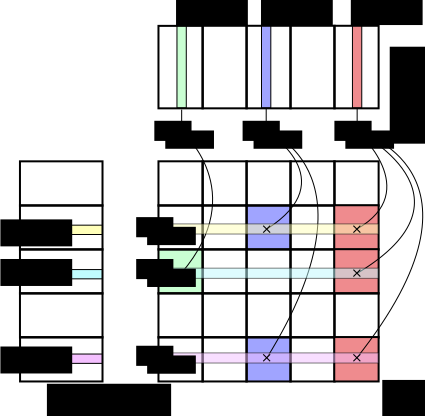
\includegraphics[width=0.8\linewidth]{figures/matrix-partition.png}
\end{figure}

\subsection{Partitioning} \label{sec:partitioning}

%This effectively defines a 2D uniform checkerboard partition of $\Am$ with matrix blocks $\Am_{(r,c)} = \Am(I_r, J_c)$ for all $1 \le r \le P_r$ and $1 \le c \le P_c$, as well as a row partition of $\Wm$ and $\Hm$.
%Here, process $p$ owns the matrix subblock $\Am_{(r, c)}$, where $r = \lfloor P/P_c \rfloor + 1$ and $c = (P \mod P_c) + 1$, as well as $m / P$ and $n / P$ rows of $\Wm(I_r, :)$ and $\Hm(J_c, :)$.
%

\Cref{alg:distnmf} requires a partitioning of the nonzeros of $\Am$ as well as the rows and the columns of $\Wm$ and $\Hm$, and these three partitions completely determine its computational and communication costs.
Here, we compare different partitioning strategies, employed by \mpifaun, \hypertensor, and SpMV kernels, and argue how they relate to these two performance metrics.

%Our algorithm is fine-grained; meaning that it can work any fine-grain, 1D, or 2D/checkerboard partition of the sparse matrix $\Am$.
%Here, however, we exclusively focus on $P_r \times P_c$~(where $P = P_r P_c$) checkerboard partitionings, and always set $P_c$ to the number of cores available per compute node in the cluster.
%This helps us reduce the communication cost in two ways.
%The first one corresponds to that we do not employ shared-memory parallelism in our implementation, hence assign one MPI rank per core.
%In this scenario, by assigning each group of $P_c$ processes owning the same row block of $\Am$ to the same node, and similarly assigning the corresponding row blocks of $\Wm$ and $\Wmt$ to these processes, we effectively eliminate the communication in the row dimension of the process grid~(which pertains to communicating matrices $\Wm$ and $\Wmt$) as these row exchanges stay within a node.
%This enables us to focus solely on reducing the communication due to columns of $\Hm$ and $\Hmt$.
%Second, this topology bounds the maximum number of messages sent per process by $P_r-1$ and $P_c-1$, thereby significantly reduce the communication latency by a factor of $P_c$ in compare with a fine-grain or a 1D partition, which incurs up to $P-1$ messages per process.

\subsubsection{Partitioning $\Am$} \label{sec:cp1d}

\paragraph{Checkerboard hypergraph partitioning~(\textbf{CH2})}
A hypergraph consists of vertices with associated weights and hyperedges that connect two or more vertices.
In the literature, a hypergraph is typically formed by adding a vertex for each computational task with the associated execution cost, adding a hyperedge for each data element, and connecting the vertex to a hyperedge whenever the associated task and the data are dependent.
Then, the vertices of the hypergraph is partitioned using a hypergraph partitioner to distribute vertex loads to parts equitably while reducing a metric called \emph{cutsize}, which amounts to minimizing the total number of different parts each hyperedge connects.
This corresponds in the actual computation to minimizing the data dependencies between tasks, hence the communication volume.

Traditional checkerboard hypergraph partitioning aims to partition the matrix $\Am$ into $P_r$ row slices first, and $P_c$ column slices next to obtain an $P_r \times P_c$ checkerboard partition~\cite{caay:99,aycu:08}.
The first partitioning phase is done using a column-net hypergraph model, in which for each row $\Am(i, :)$, a vertex $v_i$ with weight equaling to the number of nonzeros in $\Am(i, :)$ is created.
Each column $j$ is represented with a hyperedge $h_j$ and for each nonzero $(i, j) \in \Am$, which implies a dependency to $\Hm(:, j)$ in computing $\Wmt(i, :)$ at \cref{line:ah}, we connect $v_i$ to $h_j$.
This hypergraph is partitioned into $P_r$ parts giving the row partition of the checkerboard topology.
The second partitioning phase uses a row-net hypergraph model induced by this row partition, where each column is represented with a vertex with $P_r$ weights corresponding to the number of nonzeros in that column in all $P_r$ row segments.
Partitioning this hypergraph into $P_c$ parts finalizes the $P_r \times P_c$ checkerboard partitionin by balancing the weights~(number of nonzeros of $\Am_{(r, c)}$) of each part while minimizing the communication volume.
In the context of NMF, one issue arises when the matrix has some variance in the number of nonzeros in its rows/columns, which in turns yields unbalanced row/column strides.
This in turn creates an imbalance in the NNLS computations as rows/cols of $\WW$/$\HH$ are partitioned to the processes in the same stride.
To alleviate this issue, we modify this scheme slightly as follows.
In both row and column partitioning phases, we add an additional constant weight to vertices.
Balancing this additional constraint in hypergraph partitioning is expected to prevent such imbalanced strides.
This partitioning model~(which we call \textbf{CH2}) succesfully grasps the computation~(both SpMM and NNLS) and communication requirements using checkerboard topology for sparse NMF, yet is costly to compute in practice due to high number of constraints~($P_r + 1$) in the row-net hypergraph.

%We assign the value $(nnz(\Am) / m + nnz(\Am(i, :))$ to each vertex $v_i$.
%This weighting is preferred to find a tradeoff between balancing the number of vertices, which corresponds to the cost of dense matrix operations, and balancing the number of nonzeros per part, which corresponds to the cost of sparse matrix-dense matrix multiplication.
%We establish these two load balance goals by assigning a fixed cost to each vertex in the first summand, and increasing the cost of the vertices corresponding to denser rows in the second summand.
%We then partition this hypergraph into $R$ parts by balancing the vertex weights, and minimizing the cutsize of the hypergraph.
%In \cref{fig:partition} we also show this hypergraph construction for a $3 \times 3$ subset of the $A$ where rows corresponding to each vertex are highlighted and connected to related hyperedges.
%In this partitioning, minimizing the cutsize of this hypergraph exactly corresponds to minimizing the total communication volume due to columns of $\Hm$ and $\Hmt$ as is clear in \cref{fig:partition}, whereas balancing the vertex weights corresponds to balancing the cost of sparse matrix-dense matrix multiplications as well as dense matrix operations in computing Gram matrices and $\textsc{Nnls}$ in each process row.

%Once the matrix is partitioned into $R$ row slices, one can similarly partition columns of $\Am$ into $C$ parts using a multi-constraint formulation~\cite{aycu:08} using a \emph{row-net} hypergraph.
%Yet in our case, we skip this common approach for two reasons.
%First, existing multi-constraint partitioning tools are known to be not as efficient nor effective as single-constraint partitioners in practice.
%Second, the main goal of hypergraph partitioning of columns is to minimize the communication volume due to rows, whereas in our case communication of rows of $\Wm$ and $\Wmt$ stays within a node with a proper mapping of processes, and this communication cost would be negligible.
%Therefore, we instead partition columns randomly, which is expected to provide balance the number of nonzeros of $\Am$, number of columns of $\Hm$ and $\Hmt$, the amount of column communication volume due to columns of $\Hm$ and $\Hmt$.

\paragraph{1D-like checkerboard hypergraph partitioning~(\textbf{CH1})}
This variant partitions rows same as $\textbf{CH2}$, then partitions columns randomly to avoid multi-constraint partitioning.
Random column partition provides load and communication balance yet increases the communication volume for the rows of $\WW$.

\paragraph{Randomized checkerboard partitioning(\textbf{CRD})}
This scheme corresponds to partitioning both the rows and the columns of $\Am$ into $P_r$ and $P_c$ segments randomly.
It is expected to provide good load and communication balance both in sparse and dense matrix operations, but it overlooks the communication volume.

\paragraph{Uniform checkerboard partitioning(\textbf{CN})}
This partitioning variant forms an $P_R \times P_C$ partition of $\Am$ by putting a contiguous set of $m / P_R$ and $n / P_C$ rows and columns in each slice.
$\Wm$ and $\Hm$ are partitioned conformally with this topology; each process is assigned a contiguous set of  $m / P_R P_C$ and $n / P_R P_C$ rows and columns of $\Wm$ and $\Hm$.
This is the partitioning scheme employed by $\mpifaun$~\cite{KBP16, KBP16MPIFAUN}.
It provides perfect balance in NNLS step yet may incur high communication cost.
We also use a randomized variant (\urp) of this scheme in which the rows and columns of $\Am$ are permuted randomly to balance its nonzeros among parts.

\paragraph{Fine-grain hypergraph partitioning~(\textbf{FH})}
This is the partitioning strategy employed by \hypertensor.
It forms a fine-grain hypergraph involving a vertex for each nonzero $(\Am(i, j)$ and a hyperedge for each row and column index $i = 1, \dots, m$ and $j = 1, \dots, n$.
The resulting hypergraph is typically very large and is costly to partition, and unlike checkerboard variants fingerprint of processes are not restricted to a row/column stride.


\subsubsection{Partitioning $\Wm$ and $\Hm$}
Once $\Am$ is partitioned, one has to partition rows and columns of factor matrices to form the sets $\Ip$ and $\Jp$ in \cref{alg:distnmf}.
In doing so, we are interested in assigning rows and columns to processes equitably.
For this purpose, we specify imbalance parameters $\alpha$ that correspond to maximum imbalance we allow in this partitioning; i.e., $|\Ip| \le \alpha m / P$ and $|\Jp| \le \alpha n / P$ for each process $p$, and set $\alpha = 1.05$ in the experiments.

Next, for each row and column of $\Wm$ and $\Hm$ we create a list of processes that has a dependency to that row or column, which corresponds to processes owning the matrix blocks of same color in \cref{fig:partition}.
Finally, we randomly assign each row and column to one of the processes satisfying the imbalance constraint in this list.
If all processes in the list are overloaded, we assign it to the process that has the minimum number of rows/columns assigned.
For a checkerboard partition, the minimum is always chosen from the same processor row/column so that 2D communication topology is not disturbed.
Note that such an assignment increases the communication volume due to that row or column by 1; hence, in general smaller imbalance parameters yield larger communication volume due to increasing this type of assignment.
On the other hand, we desire to keep $\alpha$ small as it pertains to the load imbalance in the NNLS step.

%%\newcommand{\smaller}{\scriptsize}
%\begin{table*}[t!]
%\begin{center}
%\begin{tabular}{|c|c|c|c|c|}
%\hline
%\textbf{Algorithm} & \textbf{Flops} & \textbf{Words} & \textbf{Messages} & \textbf{Memory}  \\ \hline
%\smaller \mpifaun ($m/p < n$) & \smaller $O(2*nnz_p*k)+\frac{(m+n)k^2}{p}+F\lt(\frac mp,\frac np,k\rt)$ & \smaller $O\lt( \sqrt{\frac{mnk^2}{p}}\rt)$ & \smaller $O(\log p)^*$ & \smaller $O\lt(\frac{mn}{p}+\sqrt{\frac{mnk^2}{p}}\rt)$ \\ \hline
%\end{tabular}
%\normalsize
%\end{center}
%\caption{Leading order algorithmic costs for \NaiveAlg{} and \ParNMF{} (per iteration).  
%The function $F(\cdot)$ denotes the number of flops required for the particular NMF algorithm's Local Update Computation, aside from the matrix multiplications common across AU-NMF algorithms. \\
%$^*$The stated latency cost assumes no communication is required in \LUC; \HALS\ requires $k\log p$ messages for normalization steps.}
%\label{tab:costs}
%\end{table*}%


\section{Experiments}
\label{sec:experiment}
\newcommand{\NLS}{LUC }

In this section, we describe our implementation of \ParNMF\ and evaluate its performance.
We identify a few synthetic and real world data sets to experiment with \ParNMF\ with dimensions that span from hundreds to millions. 
We compare the performance and exploring scaling behavior of different NMF algorithms -- \MU, \HALS, and ANLS/BPP (\BPP), implemented using the parallel \ParNMF\ framework.  
The code and the  datasets used for conducting the experiments can be downloaded from \url{https://github.com/ramkikannan/nmflibrary}. 

\subsection{Experimental Setup}

\subsubsection{Data Sets}\label{sec:datasets}

We used sparse and dense matrices that are either synthetically generated or from real world applications. We explain the data sets in this section.

\begin{itemize}
\item Dense Synthetic Matrix: We generate a low rank matrix as the product of two uniform random matrices of size 207,360 $\times$ 100 and 100 $\times$ 138,240. 
The dimensions of this matrix are chosen to be evenly divisible for a particular set of processor grids.  
\item Sparse Synthetic Matrix: We generate a random sparse Erd\H{o}s-R\'{e}nyi matrix of the size 207,360 $\times$ 138,240 with density of 0.001.  That is, every entry is nonzero with probability 0.001.
\item Dense Real World Matrix ({\em Video}):  NMF is used on video data for background subtraction in order to detect moving objects. The low rank matrix $\hat{\AA} = \WW \HH$ represents background and the error matrix $\AA - \hat{\AA}$ represents moving objects.  %Detecting moving objects has many real-world applications such as traffic estimation \cite{Fujimoto2014} and security monitoring \cite{BSJJZ2015}.
In the case of detecting moving objects in streaming videos, the last several minutes of video is taken from the live video camera to construct the non-negative matrix. 
An algorithm to incrementally adjust the NMF based on the streaming video is presented in \cite{kim2013nonnegative}. 
To simulate this scenario, we collected a video in a busy intersection of the Georgia Tech campus at 20 frames per second. 
From this video, we took video for approximately 12 minutes and  then reshaped the matrix such that every RGB frame is a column of our matrix, so that the matrix is dense with size 1,013,400 $\times$ 13,824. 
\item Sparse Real World Matrix ({\em Webbase}): This data set is a directed sparse graph whose nodes correspond to webpages (URLs) and edges correspond to hyperlinks from one webpage to another.
The NMF output of this directed graph helps us understand clusters in graphs.
We consider two versions of the data set: {\em webbase-1M} and {\em webbase-2001}.
The dataset webbase-1M contains about 1 million nodes (1,000,005) and 3.1 million edges (3,105,536), and was first reported by Williams et al. \cite{Williams2009}.  
The version webbase-2001 has about 118 million nodes (118,142,155) and over 1 billion edges (1,019,903,190); it was first reported by Boldi and Vigna  \cite{Boldi2004}.  
Both data sets are available in the University of Florida Sparse Matrix Collection \cite{DH11} and the latter {\em webbase-2001} being the largest among the entire collection.
\item Text data ({\em Stack Exchange}): 
Stack Exchange is a network of question-and-answer websites on topics in varied fields, each site covering a specific topic, where questions, answers, and users are subject to a reputation award process. There are many Stack Exchange forums, such as {\em ask ubuntu, mathematics, latex}. 
We downloaded the latest anonymized dump of all 
user-contributed content on the Stack Exchange network from \cite{stkxchngdataset}. 
%Each site is formatted as a separate archive consisting of XML files zipped via 7-zip using bzip2 compression. 
%Each site archive includes Posts, Users, Votes, Comments, PostHistory and PostLinks. 
%For complete schema information, see the included readme.txt. 
We used only the questions from the most popular site called Stackoverflow and did not include the answers and comments. 
We removed the standard 571 English stop words (such as {\em are, am, be, above, below}) and then used snowball stemming available through the Natural Language Toolkit (NLTK) package \cite{LB2002}.
After this initial pre-processing, we deleted HTML tags (such as {\em lt, gt, em}) from the posts. 
The resulting bag-of-words matrix has a vocabulary of size 627,047 over 11,708,841 documents with 365,168,945 non-zero entries. 
In this data, the vocabulary is larger than the typical set of English words because it includes variables, constants, and other programming constructs of various programming languages from the user questions.
%We ran NMF on this dataset for finding 50 topics whose sample topic words are presented at the end of this section. 
\end{itemize}

The size of all the real world data sets were adjusted to the nearest size for uniformly distributing the matrix. 

\subsubsection{Implementation Platform}

We conducted our experiments on ``Rhea'' at the Oak Ridge Leadership Computing Facility (OLCF).
Rhea is a commodity-type Linux cluster with a total of 512 nodes and a 4X FDR Infiniband interconnect.
Each node contains dual-socket 8-core Intel Sandy Bridge-EP processors and 128 GB of memory.
Each socket has a shared 20MB L3 cache, and each core has a private 256K L2 cache. 

%\grey{Do we want to start using the acronym for our software and discuss it here? We will park this for camera ready}

Our objective of the implementation is using open source software as much as possible 
to promote reproducibility and reuse of our code.
The entire C++ code is developed using the matrix library Armadillo \cite{sanderson2010}. 
In Armadillo, the elements of the dense matrix are stored in column major order and the sparse matrices in Compressed Sparse Column (CSC) format.
For dense BLAS and LAPACK operations, we linked Armadillo with Intel MKL -- the default LAPACK/BLAS library in RHEA. It is also easy to link Armadillo with OpenBLAS \cite{xianyi2015}. 
We use Armadillo's own implementation of sparse matrix-dense matrix multiplication, the default GNU C++ Compiler (g++ (GCC) 4.8.2) and MPI library (Open MPI 1.8.4)  on RHEA.  We chose the commodity cluster with open source software so that the numbers presented here are representative of common use. 

%\grey{Need to update this last phrase with compilation setup on Rhea}. 

\subsubsection{Algorithms}

In our experiments, we considered the following algorithms: 
\begin{itemize}
	\item \MU: \ParNMF\ (Algorithm \ref{alg:2D}) with MU (Equation \eqref{eqn:muupdate})
	\item \HALS: \ParNMF\ (Algorithm \ref{alg:2D}) with HALS (Equation \eqref{eqn:halsupdate})
	\item \BPP: \ParNMF\ (Algorithm \ref{alg:2D}) with BPP (Section \ref{sec:BPP})
	\item \Naive: \NaiveAlg\ (Algorithm \ref{alg:naive}, Section \ref{sec:naive})
\end{itemize}

Our implementation of \Naive\ (Algorithm \ref{alg:naive}) uses BPP but can be easily to extended to \MU, \HALS, and other NMF algorithms. 
%A detailed comparison of \NaiveAlg\ with \ParNMF\ is made in our earlier work \cite{KBP16}. 
%We include some benchmark results from \Naive\ to reiterate the point that communication efficiency is key to obtaining reasonable performance, but we also omit other \Naive\ results in order to focus attention on comparisons among other algorithms.

For the algorithms based on \ParNMF, we use the processor grid that is closest to the theoretical optimum (see Section \ref{sec:alg:comm}) in order to minimize communication costs.
See Section \ref{sec:procgrid} for an empirical evaluation of varying processor grids for a particular algorithm and data set.

%We choose these three algorithms to confirm the following conclusions from the analysis of Section \ref{sec:parNMF}: the performance of a naive parallelization of \NaiveAlg\ (Algorithm \ref{alg:naive}) will be severely limited by communication overheads, and the correct choice of processor grid within Algorithm \ref{alg:2D} is necessary to optimize performance.
%To demonstrate the latter conclusion, we choose the two extreme choices of processor grids and test some data sets where a 1D processor grid is optimal (e.g., the Video matrix) and some where a squarish 2D grid is optimal (e.g., the Webbase matrix).

To ensure fair comparison among algorithms, the same random seed is used across different methods appropriately. 
That is, the initial random matrix $\HH$ is generated with the same random seed when testing with 
different algorithms (note that $\WW$ need not be initialized). 
In our experiments, we use number of iterations as the stopping criteria for all the algorithms.

%\grey{Need to update the following paragraph for our running times, maybe consider moving it elsewhere...}
While we would like to compare against other high-performance NMF algorithms in the literature, the only other distributed-memory implementations of which we're aware are implemented using Hadoop and are designed only for sparse matrices \cite{liao2014cloudnmf},
\cite{liu2010distributed}, \cite{gemulla2011large}, \cite{Yin2014} and \cite{Faloutsos2014}.
We stress that Hadoop is not designed for high performance computing of iterative numerical 
algorithms, requiring disk I/O between steps, so a run time comparison between a Hadoop 
implementation and a C++/MPI implementation is not a fair comparison of parallel algorithms.
A qualitative example of differences in run time is that a Hadoop implementation of the MU algorithm on 
a large sparse matrix of size $2^{17} \times 2^{16}$ with $2 \times {10^8}$ nonzeros (with k=8) 
takes on the order of 50 minutes per iteration \cite{liu2010distributed}, while our MU implementation 
takes 0.065 seconds per iteration for the synthetic data set (which is an order of magnitude larger in 
terms of rows, columns, and nonzeros) running on only 16 nodes. 
%Based on our survey, we are the fastest distributed NMF algorithm in the literature. 

% input file with plotting macros
% !TEX root = experiments.tex

% macros for plotting
\newcommand{\datafile}{}
\newcommand{\alg}{}
\newcommand{\numiterations}{30}
\newcommand{\minvalue}{1}

% toggles whether or not to plot naive results (if not, the rows of the data file also need to be commented out)
\newif\ifnaive
% toggles ksweep vs scaling plot
\newif\ifksweep
% toggles legend
\newif\iflegend
% toggles y axis label
\newif\ifylabel
% toggles wider plot area
\newif\ifwider


\newcommand{\setcolors}{
\pgfplotsset{cycle list={
	red, fill=red \\ 
	blue, fill=blue \\ 
	green, fill=green \\ 
	red, pattern=crosshatch, pattern color=red \\
	blue, pattern=crosshatch, pattern color=blue \\
	green, pattern=crosshatch, pattern color=green \\
}};
}

% set options for grouped bar plot
\newcommand{\breakdownplotoptions}{
	ybar stacked,
	reverse legend,
	bar width=6pt,
	width=9cm, height=3.85cm,
	ylabel={Time (seconds)}, 
	y label style={yshift=-.5cm},
	ymin=0,
	symbolic x coords={1,16,81,256},
	xtick=data,
	legend={DimTree}
}

% stacked bar plot command
\newcommand{\breakdownplot}{
\begin{axis}[\breakdownplotoptions]
	\setcolors
	\addplot table[x=p, y expr=(\thisrow{mttkrp}/(\minvalue*\numiterations))] {\datafile};
	\addplot table[x=p, y expr=(\thisrow{nnls}/(\minvalue*\numiterations))] {\datafile};
	\addplot table[x=p, y expr=(\thisrow{gram}/(\minvalue*\numiterations))] {\datafile};
	\addplot table[x=p, y expr=(\thisrow{allgather}/(\minvalue*\numiterations))] {\datafile};
	\addplot table[x=p, y expr=(\thisrow{reducescatter}/(\minvalue*\numiterations))] {\datafile};
	\addplot table[x=p, y expr=(\thisrow{allreduce}/(\minvalue*\numiterations))] {\datafile};
\end{axis}
}

% labels for bar groups (manually positioned)
\newcommand{\labels}{
%\node [align=center,text width=3cm] at (1.25cm, -.95cm)   {\ifksweep 10 \else 16 \fi};
%\node [align=center,text width=3cm] at (3cm, -0.95cm)   {\ifksweep 20 \else 96 \fi};
%\node [align=center,text width=3cm] at (4.6cm, -0.95cm)   {\ifksweep 30 \else 384 \fi};
%\node [align=center,text width=3cm] at (6.3cm, -0.95cm) {\ifksweep 40 \else 864 \fi};
%\node [align=center,text width=3cm] at (8.15cm, -0.95cm) {\ifksweep 50 \else 1536 \fi};
\node [align=center,text width=3cm] at (1cm, -1.15cm)   {\ifksweep 10 \else 16 \fi};
\node [align=center,text width=3cm] at (2.4cm, -1.15cm)   {\ifksweep 20 \else 96 \fi};
\node [align=center,text width=3cm] at (3.7cm, -1.15cm)   {\ifksweep 30 \else 384 \fi};
\node [align=center,text width=3cm] at (5.1cm, -1.15cm) {\ifksweep 40 \else 864 \fi};
\node [align=center,text width=3cm] at (6.4cm, -1.15cm) {\ifksweep 50 \else 1536 \fi};
}

% allows for filtering rows from dat file
\pgfplotsset{
    discard if not/.style 2 args={
        x filter/.append code={
            \edef\tempa{\thisrow{#1}}
            \edef\tempb{#2}
            \ifx\tempa\tempb
            \else
                \def\pgfmathresult{inf}
            \fi
        }
    }
}

% set options for strongscaling plot
\newcommand{\strongscalingplotoptions}{
	log basis y={2},
	log basis x={2},
	xlabel=Nodes,
	ylabel=Time (s),
	y tick label style={
        /pgf/number format/.cd,
            precision=4,
	},
	legend style={draw=none, cells={align=left}, nodes={scale=0.7}}
}

% plot time over p, filtering rows out appropriately
\newcommand{\strongscalingplot}{
\begin{loglogaxis}[\strongscalingplotoptions]
	%\addplot+ [discard if not={algo}{liavas},thick,mark options={solid}] table [x={nodes}, y={totaltime}] {\datafile};
	%\addplot+ [discard if not={algo}{nodimtree},thick,mark options={solid},mark=square*] table [x={nodes}, y={totaltime}] {\datafile};
	\addplot+ [discard if not={alg}{D},thick,mark options={solid},mark=triangle*] table [x={p}, y={total}] {\datafile};
	\legend{DimTree}
\end{loglogaxis}
}



\subsection{Relative Error over Time} \label{sec:convergence}

There are various metrics to compare the quality of the 
NMF algorithms \cite{kim2013nonnegative}. The most common among these metrics are (a) relative error and (b) projected 
gradient. The former represents the closeness of the low rank approximation $\hat{\AA}\approx\WW\HH$, which is generally the optimization objective. 
The latter 
represent the quality of the produced low rank factors and the stationarity of the final solution. These 
metrics are also used as the stopping criterion for terminating the iteration of the NMF algorithm as in 
line \ref{algo:nmfloop} of Algorithm \ref{alg:aunmf}. Typically a combination of the number of iterations 
along with improvement of these metrics until a tolerance is met is used as stopping criterion. In this paper, we use 
relative error for the comparison as it is monotonically decreasing, as opposed to projected gradient of the 
low rank factors, which shows oscillations over iterations. The relative error can be formally defined as 
$\|\AA-\WW\HH\|_F/\|\AA\|_F$. 

In Figure \ref{fig:convergence}, we measure the relative error at the end of every iteration (i.e., after the updates of both $\WW$ and $\HH$) for all three algorithms \MU, \HALS, and 
\BPP, and we plot the relative error over time (each mark represents an iteration).
We consider three real world datasets, \emph{video}, \emph{stack exchange} and \emph{webbase-1M}, and set $k=50$. 
We used only the number of iterations as stopping criterion and,  
just for this section, ran all the algorithms for 30 iterations. 
We note that the convergence behavior and computed factors can vary over different initializations; we used the same initial values across all three algorithms in these experiments.
Also, we observed that for these data sets, the convergence behavior was not sensitive to initialization (the final residual errors varied by less than 1\% in our experiments).
NMF solutions are guaranteed to be unique in certain cases, with mild assumptions on the input data \cite{BLRG14,HFS2016}, but we do not check those assumptions for these datasets.

To begin with, we explain the observations on the dense \emph{video} dataset presented in Figure \ref{fig:denserwerr}. 
The relative error of \MU\ is highest at 0.1812 after 30 iterations and \HALS's is the least with 0.1273; \BPP's relative error
is  0.1716 after 30 iterations. 
%For this data, although the per-iteration times vary across algorithms and \BPP\ has the longest per-iteration time, it converged more quickly than \HALS\ or \MU\ because it solves subproblems exactly.
%From the figure, we can observe that \BPP\  error didn't change after 29 iterations where as \HALS\ and \MU\ was still improving marginally at the 4th decimal even after 30 iterations.  

We can observe that the relative error of \emph{stack exchange} from Figure \ref{fig:stackexchangeerr} is better 
than \emph{webbase-1M} from Figure \ref{fig:sparserwerr} over all three algorithms. 
In the case of the \emph{stack exchange} dataset, the relative errors after 30 iterations follow the pattern \MU\ $>$ \HALS\ $>$ \BPP, with values 0.8509, 0.8395, and 0.8377 respectively. 
%Unlike the \emph{video} dataset, both \MU\ and \HALS\ stopped improving after 23 iterations, 
%where as \BPP\ was still improving in the 4th decimal even though its error was better than the others. 
However, the difference in relative error for the \emph{webbase-1M} dataset is negligible, though the relative ordering of \MU\ $>$ \HALS\ $>$ \BPP\ is consistent, with values of 0.99927 for \MU\, 0.99920 for \HALS\ and 0.99919 for \BPP. 

In general, for these datasets \BPP\ identifies better approximations and converges faster than \MU\ and \HALS\ despite the extra per-iteration time, which is consistent with the 
literature \cite{kim2013nonnegative,kim2011fast}. 
However, for the sparse datasets, the differences in relative error are small across the NMF algorithms. 

%The Figure \ref{fig:stackexchangerr} shows the comparison of these algorithms on the stack exchange dataset explained in Section \ref{sec:datasets}. 

%\captionsetup[subfigure]{labelfont=normalfont,textfont=normalfont,singlelinecheck=off,justification=raggedright}

\begin{figure}

% set which run to plot
\renewcommand{\run}{3}

\begin{subfigure}{0.3 \columnwidth}
\ylabeltrue
\begin{tikzpicture}
\renewcommand{\datafile}{data/denserwerr-time.dat}
\renewcommand{\run}{1}
\relerrplot
\renewcommand{\run}{3}
\end{tikzpicture}
\ylabelfalse
\subcaption{Video}
\label{fig:denserwerr}
\end{subfigure}
~
\begin{subfigure}{0.3 \columnwidth}
\begin{tikzpicture}
\renewcommand{\datafile}{data/stkx-5runs-err.dat}
\legendtrue
\relerrplot
\legendfalse
\end{tikzpicture}
\subcaption{Stack Exchange}
\label{fig:stackexchangeerr}
\end{subfigure}
~
\begin{subfigure}{0.3 \columnwidth}
\begin{tikzpicture}
\renewcommand{\datafile}{data/webbase1M-5runs-err.dat}
\relerrplot
\end{tikzpicture}
\subcaption{Webbase}
\label{fig:sparserwerr}
\end{subfigure}

\caption{Relative error comparison of \MU, \HALS, \BPP\ on real world datasets.}
\label{fig:convergence}
\end{figure}

\subsection{Time Per Iteration}

In this section we focus on per-iteration time of all the algorithms.
We report four types of experiments, varying the number of processors (Section \ref{sec:scaling}), the rank of the approximation (Section \ref{sec:ksweep}), the shape of the processor grid (Section \ref{sec:procgrid}), and scaling up the dataset size.
For each experiment we report a time breakdown in terms of the overall computation and communication steps (described in Section \ref{sec:perf-breakdown}) shared by all algorithms.

\subsubsection{Time Breakdown}
\label{sec:perf-breakdown}

To differentiate the computation and communication costs among the algorithms, we present the time breakdown among the various tasks within the algorithms for all performance experiments.
For Algorithm \ref{alg:2D}, there are three local computation tasks and three communication tasks to compute each of the factor matrices:
\begin{itemize}
	\item \textbf{MM}, computing a matrix multiplication with the local data matrix and one of the factor matrices;
	\item \textbf{\LUC}, local updates either using \BPP\ or applying the remaining work of the \MU\ or \HALS\ updates (i.e., the total time for both $UpdateW$ and $UpdateH$ functions); 
	\item \textbf{Gram}, computing the local contribution to the Gram matrix;
	\item \textbf{All-Gather}, to compute the global matrix multiplication;
	\item \textbf{Reduce-Scatter}, to compute the global matrix multiplication;
	\item \textbf{All-Reduce}, to compute the global Gram matrix.
\end{itemize}
In our results, we do not distinguish the costs of these tasks for $\WW$ and $\HH$ separately; we report their sum, though we note that we do not always expect balance between the two contributions for each task.
Algorithm \ref{alg:naive} performs all of these tasks except Reduce-Scatter and All-Reduce; all of its communication is in All-Gather.

\subsubsection{Scaling \texorpdfstring{$p$}{p}: Strong Scaling}
\label{sec:scaling}

Figure \ref{fig:scaling} presents a strong scaling experiment with four data sets: \emph{sparse synthetic}, \emph{dense synthetic}, \emph{webbase-1M}, and \emph{video}.
In this experiment, for each data set and algorithm, we use low rank $k=50$ and vary the number of processors (with fixed problem size).
We use $\{1,6,24,54,96\}$ nodes; since each node has 16 cores, this corresponds to $\{16,96,384,864,1536\}$ cores.
We report average per-iteration times.

We highlight three main observations from these experiments:
\begin{enumerate}
	\item \label{obs:1} \Naive\ is slower than all other algorithms for large $p$;
	\item \label{obs:2} \MU, \HALS, and \BPP\ (algorithms based on \ParNMF) scale up to over 1000 processors;
	\item \label{obs:3} the relative per-iteration cost of \LUC\ decreases as $p$ increases (for all algorithms), and therefore the extra per-iteration cost of \BPP\ (compared with \MU\ and \HALS) becomes negligible.
\end{enumerate}

\paragraph{Observation \ref{obs:1}} 
%We report \Naive\ performance only for the synthetic data sets (Figures \ref{fig:sparsesynstrongscale} and \ref{fig:densesynscaling}); the results for the real-world data sets are similar.
For the Sparse Synthetic data set, \Naive\ is $4.2\times$ slower than the fastest algorithm (\BPP) on 1536 processors; for the Dense Synthetic data set, \Naive\ is $1.6\times$ slower than the fastest algorithm (\MU) at that scale.
The slowdown increases to $7.7\times$ and $3.6\times$ for the sparse and dense real-world datasets, respectively.
Nearly all of this slowdown is due to the communication costs of \Naive.
Theoretical and practical evidence supporting the first observation is also reported in our previous paper \cite{KBP16}.
However, we also note that \Naive\ is the fastest algorithm for the smallest $p$ for each problem, which is largely due to reduced MM time.
Each algorithm performs exactly the same number of flops per MM; the efficiency of \Naive\ for small $p$ is due to cache effects.
For example, for the Dense Synthetic problem on 96 processors, the output matrix of \Naive's MM fits in L2 cache, but the output matrix of \ParNMF's MM does not; these effects disappear as $p$ increases.

\paragraph{Observation \ref{obs:2}}
Algorithms based on \ParNMF\ (\MU, \HALS, \BPP) scale well, up to over 1000 processors.
All algorithms' run times decrease as $p$ increases, with the exception of the Sparse Real World data set, in which case all algorithms slow down scaling from $p=864$ to $p=1536$ (we attribute this lack of scaling to load imbalance).
For sparse problems, comparing $p=16$ to $p=1536$ (a factor increase of 96), we observe speedups from \BPP\ of $59\times$ (synthetic) and $22\times$ (real world).
For dense problems, comparing $p=96$ to $p=1536$ (a factor increase of 16), \BPP's speedup is $12\times$ for both problems.
\MU\ and \HALS\ demonstrate similar scaling results.
For comparison, speedups for \Naive\ were $8\times$ and $3\times$ (sparse) and $6\times$ and $4\times$ (dense).

\paragraph{Observation \ref{obs:3}}
\MU, \HALS, and \BPP\ share all the same subroutines except those that are characterized as \LUC.
Considering only \LUC\ subroutines, \MU\ and \HALS\ require fewer operations than \BPP. However, \HALS\ has to make one additional communication for normalization of $\WW$. 
For small $p$, these cost differences are apparent in Figure \ref{fig:scaling}.
For example, for the sparse real world data set on 16 processors, \BPP's \LUC\ time is $16\times$ that of $\MU$, and the per iteration time differs by a factor of $4.5$.
However, as $p$ increases, the relative time spent in \LUC\ decreases, so the extra time taken by \BPP\ has less of an effect on the total per iteration time.
By contrast, for the dense real world data set on 1536 processors, \BPP\ spends a factor of 27 times more time in \LUC\ than \MU\ but only $11\%$ longer over the entire iteration.
For the synthetic data sets, \LUC\ takes $24\%$ (sparse) on 16 processors and $84\%$ (dense) on 96 processors, and that percentage drops to $11\%$ (sparse) and $15\%$ (dense) on 1536 processors.

These trends can also be seen theoretically (Table \ref{tab:costs}).
We expect local computations like MM, \LUC, and Gram to scale like $1/p$, assuming load balance is preserved.
If communication costs are dominated by the number of words being communicated (i.e., the communication is bandwidth bound), then we expect time spent in communication to scale like $1/\sqrt p$, and at least for dense problems, this scaling is the best possible.
Thus, communication costs will eventually dominate computation costs for all NMF problems, for sufficiently large $p$.
(Note that if communication is latency bound and proportional to the number of messages, then time spent communicating actually increases with $p$.)

The overall conclusion from this empirical and theoretical observation is that the extra per-iteration cost of \BPP\ over alternatives like \MU\ and \HALS\ decreases as the number of processors $p$ increases.
As shown in Section \ref{sec:convergence} the faster error reduction of \BPP\ typically reduces the overall time to solution compared with the alternatives even it requires more time for each iteration.
Our conclusion is that as we scale up $p$, this tradeoff is further relaxed so that \BPP\ becomes more and more advantageous for both quality and performance.

%\captionsetup[subfigure]{labelfont=normalfont,textfont=normalfont,singlelinecheck=off,justification=raggedright}

\begin{figure}

\naivetrue
\ksweepfalse
\legendtrue

\begin{subfigure}{\columnwidth}
%\centering
\begin{tikzpicture}
\renewcommand{\datafile}{data/sparsesynstrong_scale_pgf.dat}
\makeplot
\labels
\end{tikzpicture}
\subcaption{Sparse Synthetic}
\label{fig:sparsesynstrongscale}
\end{subfigure}
\legendfalse

\begin{subfigure}{\columnwidth}
%\centering
\begin{tikzpicture}
\renewcommand{\datafile}{data/densesynstrong_scale_pgf.dat}
\makeplot
\labels
\end{tikzpicture}
\subcaption{Dense Synthetic}
\label{fig:densesynscaling}
\end{subfigure}

%\naivefalse

\begin{subfigure}{\columnwidth}
%\centering
\renewcommand{\datafile}{data/sparserwstrong_scale_pgf.dat}
\begin{tikzpicture}
\makeplot
\labels
\end{tikzpicture}
\subcaption{Sparse Real World (webbase-1M)}
\label{fig:sparserwscaling}
\end{subfigure}

\begin{subfigure}{\columnwidth}
%\centering
\renewcommand{\datafile}{data/denserwstrong_scale_pgf.dat}
\begin{tikzpicture}
\makeplot
\labels
\end{tikzpicture}
\subcaption{Dense Real World (Video)}
\label{fig:denserwscaling}
\end{subfigure}

\caption{Per-iteration times with $k=50$, varying $p$ (strong scaling).}
\label{fig:scaling}
\end{figure}

\subsubsection{Scaling \texorpdfstring{$k$}{k}}
\label{sec:ksweep}

Figure \ref{fig:ksweep} presents an experiment scaling up the low rank value $k$ from 10 to 50 with each of the four data sets.
In this experiment, for each data set and algorithm, the problem size is fixed and the number of processors is fixed to $p=864$.
As in Section \ref{sec:scaling}, we report the average per-iteration times.
%We also omit \Naive\ data for the real world data sets to highlight the comparisons among \MU, \HALS, and \BPP.

We highlight two observations from these experiments:
\begin{enumerate}
	\item \label{obs:a} \Naive\ is plagued by communication time that increases linearly with $k$;
	\item \label{obs:b} \BPP's time increases more quickly with $k$ than those of \MU\ or \HALS;
\end{enumerate}

\paragraph{Observation \ref{obs:a}} 
We see from the synthetic data sets (Figures \ref{fig:sparsesynksweep} and \ref{fig:densesynksweep}) that the overall time of \Naive\ increases more rapidly with $k$ than any other algorithm and that the increase in time is due mainly to communication (All-Gather).
Table \ref{tab:costs} predicts that \Naive\ communication volume scales linearly with $k$, and we see that in practice the prediction is almost perfect with the synthetic problems.
This confirms that the communication is dominated by bandwidth costs and not latency costs (which are constant with respect to $k$).
We note that the communication cost of \ParNMF\ scales like $\sqrt k$, which is why we don't see as dramatic an increase in communication time for \MU, \HALS, or \BPP\ in Figure \ref{fig:ksweep}.

\paragraph{Observation \ref{obs:b}}
 Focusing attention on time spent in \NLS computations, we can compare how \MU, \HALS, and \BPP\ scale differently with $k$.
 We see a more rapid increase of \NLS time for \BPP\ than \MU\ or \HALS; this is expected because the \NLS computations unique to \BPP\ require between $O(k^3)$ and $O(k^4)$ operations (depending on the data) while the unique \NLS computations for \MU\ and \HALS\ are $O(k^2)$, with all other parameters fixed.
%It is generally observed that in both dense and sparse datasets, higher the low rank $k$ lesser the error \cite{kim2011fast}. For eg., the relative error of NMF algorithm with low rank $k=10$ will be more than the low rank $k=50$. 
Thus, the extra per-iteration cost of \BPP\ increases with $k$, so the advantage of \BPP\ of better error reduction must also increase with $k$ for it to remain superior at large values of $k$.
%\grey{can we confirm this in convergence section?}
We also note that although the number of operations within MM grows linearly with $k$, we do not observe much increase in time from $k=10$ to $k=50$; this is due to the improved efficiency of local MM for larger values of $k$.

\begin{figure}

\naivetrue
\ksweeptrue
\legendtrue

\begin{subfigure}{\columnwidth}
%\centering
\renewcommand{\datafile}{data/sparsesyn864_ksweep_scale_pgf.dat}
\begin{tikzpicture}
\makeplot
\labels
\end{tikzpicture}
\subcaption{Sparse Synthetic}
\label{fig:sparsesynksweep}
\end{subfigure}
\legendfalse

\begin{subfigure}{\columnwidth}
%\centering
\renewcommand{\datafile}{data/densesyn864_ksweep_scale_pgf.dat}
\begin{tikzpicture}
\makeplot
\labels
\end{tikzpicture}
\subcaption{Dense Synthetic}
\label{fig:densesynksweep}
\end{subfigure}

%\naivefalse

\begin{subfigure}{\columnwidth}
%\centering
\renewcommand{\datafile}{data/sparserwksweep_scale_pgf.dat}
\begin{tikzpicture}
\makeplot
\labels
\end{tikzpicture}
\subcaption{Sparse Real World (webbase-1M)}
\label{fig:sparserwksweep}
\end{subfigure}

\begin{subfigure}{\columnwidth}
\renewcommand{\datafile}{data/denserw_ksweep_scale_pgf.dat}
\begin{tikzpicture}
\makeplot
\labels
\end{tikzpicture}
\caption{Dense Real World (Video)}
\label{fig:denserwksweep}
\end{subfigure}

\caption{Per-iteration times with $p=864$, varying low rank $k$.}
\label{fig:ksweep}
\end{figure}

\subsubsection{Varying Processor Grid}
\label{sec:procgrid}

In this section we demonstrate the effect of the dimensions of the processor grid on per-iteration performance.
%As described in Section \ref{sec:alg:comm}, Algorithm \ref{alg:2D} is correct for any $p_r$ and $p_c$, but 
For a fixed total number of processors $p$, the communication cost of Algorithm \ref{alg:2D} varies with the choice of $p_r$ and $p_c$.
To minimize the amount of data communicated, the theoretical analysis suggests that the processor grid should be chosen to make the sizes of the local data matrix as square as possible.
This implies that if $m/p > n$, $p_r=p$ and $p_c=1$ is the optimal choice (a 1D processor grid); likewise if $n/p > m$ then a 1D processor grid with $p_r=1$ and $p_c=p$ is the optimal choice.
Otherwise, a 2D processor grid minimizes communication with $p_r \approx \sqrt{mp/n}$ and $p_c \approx \sqrt{np/m}$ (subject to integrality and $p_rp_c=p$).

Figure \ref{fig:procsweep} presents a benchmark of \BPP\ for the Sparse Synthetic data set for fixed values of $p$ and $k$.
We vary the processor grid dimensions from both 1D grids to the 2D grid that matches the theoretical optimum exactly.
Because the sizes of the Sparse Synthetic matrix are $172{,}800\times115{,}200$ and the number of processors is 1536, the theoretically optimal grid is $p_r = \sqrt{mp/n} = 48$ and $p_c = \sqrt{np/m} = 32$.
The experimental results confirm that this processor grid is optimal, and we see that the time spent communicating increases as the processor grid deviates from the optimum, with the 1D grids performing the worst.

\begin{figure}
\renewcommand{\datafile}{data/sparsesynpsweep_scale_pgf.dat}
\centering
\begin{tikzpicture}
\begin{axis}[
	ybar stacked,
	reverse legend,
	bar width=12pt,
	width=7cm, height=5cm,
	ylabel={Time (seconds)}, 
	y label style={yshift=-0.5cm},
	x label style={yshift=-0.5cm},
	ymin=0,
	symbolic x coords={1-1536,8-192,16-96,32-48,48-32,96-16,192-8,1536-1},
	xticklabels={$1{\times}1536$,$8{\times}192$,$16{\times}96$,$32{\times}48$,$48{\times}32$,$96{\times}16$,$192{\times}8$,$1536{\times}1$},
	xtick=data,
	xticklabel style={xshift=.1cm,rotate=45,anchor=east},
	xlabel={Processor Grid}, 
	%legend style={draw=none,row sep=-0.1cm},
	%legend style={at={(1,.5)},anchor=west}
	legend style={at={(0.5,1.2)},anchor=north},
	legend columns=-1,
	legend style={draw=none, cells={align=left}, nodes={scale=0.8}},
]
	\setcolors
	\addplot table[x=pg, y expr=(\thisrow{mm}/(\minvalue*\numiterations))] {\datafile};
	\addplot table[x=pg, y expr=(\thisrow{nnls}/(\minvalue*\numiterations))] {\datafile};
	\addplot table[x=pg, y expr=(\thisrow{gram}/(\minvalue*\numiterations))] {\datafile};
	\addplot table[x=pg, y expr=(\thisrow{allgather}/(\minvalue*\numiterations))] {\datafile};
	\addplot table[x=pg, y expr=(\thisrow{reducescatter}/(\minvalue*\numiterations))] {\datafile};
	\addplot table[x=pg, y expr=(\thisrow{allreduce}/(\minvalue*\numiterations))] {\datafile};
	\legend{MM, \NLS, Gram, All-Gather, Reduce-Scatter, All-Reduce};
\end{axis}
\end{tikzpicture}
\caption{Tuning processor grid for \BPP\ on Sparse Synthetic data set with $p=1536$ and $k=50$.}
\label{fig:procsweep}
\end{figure}

\subsubsection{Scaling up to Very Large Sparse Datasets}\label{sec:webbase-2001}

In this section, we test \ParNMF\ by scaling up the problem size.
While we've used \emph{webbase-1M} in previous experiments, we consider \emph{webbase-2001} in this section as it is the largest sparse data in University of Florida Sparse Matrix Collection \cite{DH11}.
The former dataset has about 1 million nodes and 3 million edges, whereas the latter dataset has over 100 million nodes and  1 billion edges (see Section \ref{sec:datasets} for more details).
Not only is the size of the input matrix increased by two orders of magnitude (because of the increase in the number of edges), but also the size of the output matrices is increased by two orders of magnitude (because of the increase in the number of nodes).

In fact, with a low rank of $k=50$, the size of the output matrices dominates that of the input matrix: $\WW$ and $\HH$ together require a total of 88 GB, while $\AA$ (stored in compressed column format) is only 16 GB.
At this scale, because each node (consisting of 16 cores) of Rhea has 128 GB of memory, multiple nodes are required to store the input and output matrices with room for other intermediate values.
As mentioned in Section \ref{sec:new_memory}, \ParNMF\ requires considerably more temporary memory than necessary when the output matrices require more memory than the input matrix.
While we were not limited by this property for the other sparse matrices, the \emph{webbase-2001} matrix dimensions are so large that we need the memories of tens of nodes to run the algorithm.
Thus, we report results only for the largest number of processors in our experiments: 1536 processors (96 nodes).
The extra temporary memory used by \ParNMF\ is a latency-minimizing optimization; the algorithm can be updated to avoid this extra memory cost using a blocked matrix multiplication algorithm.
The extra memory can be reduced to a negligible amount at the expense of more messages between processors and synchronizations across the parallel machine.
%We have not yet implemented this update.

%In the real-world, it is difficult to acquire very large dense datasets. Most of the very large dense 
%datasets will be either be image/video data or collected out of very large scientific experiments. It is 
%common in the DM/ML community to have very large sparse dataset. In this section, to benefit the Data 
%mining and machine learning community, we report the scalability of \ParNMF\ on very directed sparse 
%webgraph over 118 million nodes and nearly 1 billion edges.  In Section \ref{sec:datasets},  we 
%discussed the details of this {\em webbase-2001} dataset. 

%It can be observed from our \ParNMF\ that we hold the dense matrices $\WW, \HH, (\WW_i)_j, 
%(\HH_j)_i, \WW^T\AA$ and $\AA \HH^T$ in memory for computation. As discussed in Section 
%{\ref{sec:memory}}, the estimated per process memory footprint of all the matrices together is $O(xx)$. In the 
%case of {\em Webbase-2001},  matrix of size 118,000,000 with low rank $k=$50 over 864 process, every 
%process  required xx GB and approximately 2GB for input sparse matrix. \ramki{Grey can we discuss to fill this up. I wanted this to be consistent with the table and the section.} We were running 16 process on every node, the estimated memory per-process along with temporary allocations,  the experiment couldn't run in 54 nodes with each node having 128GB. Hence, we are reporting the wall clock time for different tasks and the error plot for {\em Webbase-2001} over 96 nodes and 1536 processors in Figure \ref{fig:webbase2001}. 

We present results for \emph{webbase-2001} in Figure \ref{fig:webbase2001}.
The average per-iteration timing results are consistent with the observations from other synthetic and real world sparse datasets as discussed in Section \ref{sec:scaling}, though the raw times are about 2 orders of magnitude larger, as expected. 
In the case of the error plot, as observed in other experiments, \BPP\ achieves smaller error (by 1\%) than other algorithms after converging; however \MU\ and \HALS\ initially outperform \BPP. 
We also see that \MU\ outperforms \HALS\ in the first 30 iterations. 
At the 30th iteration, the error for \HALS\ is still improving at the third decimal, whereas \MU's is improving at the fourth decimal. 
We suspect that over a greater number of iterations the error of \HALS\ could become smaller than that of \MU, which would be more consistent with other datasets. 

\begin{figure}
\centering
\captionsetup[subfigure]{justification=centering}
\begin{subfigure}{0.40 \columnwidth}
\renewcommand{\datafile}{data/webbase118m_pgf.dat}
%\centering
\begin{tikzpicture}
\begin{axis}[
	ybar stacked,
	reverse legend,
	bar width=16pt,
	width=1.6in, height=1.8in,
	ylabel={Time (seconds)}, 
	y label style={yshift=-.5cm, xshift=-.5cm},
	x label style={yshift=-.5cm},
	ymin=0,
	symbolic x coords={1536-0,1536-1,1536-2},
	xticklabels={MU,HALS,ABPP},
	xtick=data,
	%xticklabel style={xshift=.15cm,rotate=45,anchor=east},
	%xlabel={NMF Algorithms}, 
	%legend style={draw=none,row sep=-0.1cm},
	%legend style={at={(1,.5)},anchor=west}
	legend style={at={(0.5,1.3)},anchor=north},
	legend columns=3,
	legend style={draw=none, cells={align=left}, nodes={scale=0.5}}
]
	\setcolors
	\addplot table[x=algo, y expr=(\thisrow{mm}/30)] {\datafile};
	\addplot table[x=algo, y expr=(\thisrow{nnls}/30)] {\datafile};
	\addplot table[x=algo, y expr=(\thisrow{gram}/30)] {\datafile};
	\addplot table[x=algo, y expr=(\thisrow{allgather}/30)] {\datafile};
	\addplot table[x=algo, y expr=(\thisrow{reducescatter}/30)] {\datafile};
	\addplot table[x=algo, y expr=(\thisrow{allreduce}/30)] {\datafile};
	\legend{MM, \NLS, Gram, All-Gather, Reduce-Scatter, All-Reduce};
\end{axis}
\end{tikzpicture}
\subcaption{Time}
\end{subfigure}
~
\begin{subfigure}{0.45 \columnwidth}
\begin{tikzpicture}
\renewcommand{\run}{1}
\legendtrue
\ylabeltrue
\widertrue
\renewcommand{\datafile}{data/webbase118m-err-time.dat}
\relerrplot
\widerfalse
\end{tikzpicture}
\subcaption{Error}
\end{subfigure}
\caption{NMF comparison on \emph{webbase-2001} for $k{=}50$ on 1536 processors.}
\label{fig:webbase2001}
\end{figure}

\subsection{Interpretation of Results}

We present results from two of the real world datasets in the Supplemental Material. 
The first example shows background separation of the \emph{video} data, and the second example shows topic modeling output on the \emph{stack exchange} text dataset. The details of these datasets are presented in Section \ref{sec:datasets}. 

While the literature covers more detail about fine tuning NMF and different NMF variants for higher quality results on these two tasks, our main focus is to show how quickly we can produce baseline NMF solutions. 
In Figure 1 of the Supplemental Material, we can see the background is removed and the moving objects (e.g., cars) are visible. 
Similarly, Table 1 of Supplemental Material shows that the NMF solution discriminates among topics and and finds coherent keywords for each topic. 

%\subsubsection{Moving Object Detection of Surveillance Video Data}
%
%As explained in the Section 6.1.1, we processed 12 minutes video that is captured from a 
%busy junction in Georgia Tech to separate the background and moving objects from this video. 
%In Figure \ref{fig:videoresults}, we present some sample frames to compare the input image with the separated background and moving objects.
%The background are the results of the low rank approximation 
%$\hat{\AA}=\WW\HH$ output yielded from our \ParNMF\ algorithm and the moving objects are given by $\AA-\hat{\AA}$. 
%We can clearly see the background remains static and the moving objects (e.g., cars) are visible. 
%
%\subsubsection{Topic Modeling of Stack Exchange Data}
%We ran 
%our \ParNMF\ algorithm on this dataset, which has nearly 12 million questions from the Stack Overflow site (under Stack Exchange) to produce 50 topics. 
%The matrix $\WW$ can be interpreted as {\em vocabulary-topic} distribution and the 
%$\HH$ as {\em topic-document} distribution.  We took the top 5 words for each of the 50 topics and 
%present them in Table \ref{tab:stackexchangetopics}. Typically a good topic generation satisfies 
%properties such as (a) finding discriminative rather than common words -- capturing words that can provide 
%some information; (b) finding different topics -- the similarity between different topics should be low; 
%(c) coherence - all the words that belong to one topic should be coherent.  There are some topic quality 
%metrics \cite{NLGB2010} that capture the usefulness of topic generation algorithm.  We can  see
% NMF generated generally high-quality and coherent topics. 
% Also, each of the topics are from different domains such as 
% databases, C/C++ programming, Java programming, and web technologies like PHP and HTML. 


\section{Conclusion} \label{sec:conclusion}
\begin{itemize}
	\item We present new parallel software for distributed memory NNCP.
	\item We demonstrate consistent speed up against existing state of the art up to $2.2\times$.
	\item We extend our algorithms and software to a general number of modes.
	\item We present analysis of our parallel algorithms showing good strong and weak parallel scaling up to thousands of cores (hundreds of nodes)
\end{itemize}

% conference papers do not normally have an appendix

% use section* for acknowledgment
\ifCLASSOPTIONcompsoc
  % The Computer Society usually uses the plural form
  %\section*{Acknowledgments}
\else
  % regular IEEE prefers the singular form
  %\section*{Acknowledgment}
\fi

\newpage 


% !TEX root = paper.tex

\appendix
\label{sec:appendix}

\begin{algorithm}
\caption{$(\CPl,\epsilon) = \text{Par-NNCP}(\TA,k)$}
\label{alg:Par-NNCP-long}
\begin{algorithmic}[1]
\Require $\TA$ is an $I_1\times \cdots \times I_N$ tensor distributed across a $P_1\times \cdots \times P_N$ grid of $P$ processors, so that $\TA_{\V{p}}$ is $(I_1/P_1)\times \cdots \times (I_N/P_N)$ and is owned by processor $\V{p}=(p_1,\dots,p_N)$, $k$ is rank of approximation
\State \Comment{Initialize data}
\State $a = \text{Norm-Squared}(\TA_{\V{p}})$
\State $\alpha = \text{All-Reduce}(a,\textsc{All-Procs})$
\State $\epsilon = $ \texttt{Inf}
\For{$n=2$ to $N$}
	\State Initialize $\Mn{H}{n}_{\V{p}}$ of dimensions $(I_n/P)\times k$ 
	\State $\M[\overline]{G} = \text{Local-SYRK}(\Mn{H}{n}_{\V{p}})$
	\State $\Mn{G}{n} = \text{All-Reduce}(\M[\overline]{G},\textsc{All-Procs})$
	\State $\Mn{H}{n}_{p_n} = \text{All-Gather}(\Mn{H}{n}_{\V{p}},\textsc{Proc-Slice}(n,\VE{p}{n}))$
\EndFor
\State \Comment{Compute NNCP approximation}
\While{$\epsilon > $ \texttt{tol}}
	\State \Comment{Perform outer iteration of BCD}
	\For{$n=1$ to $N$}
	\State \Comment{Compute new factor matrix in $n$th mode}
	\State $\M[\overline]{M} = \text{Local-MTTKRP}(\TA_{p_1\cdots p_N},\{\Mn{H}{i}_{p_i}\},n)$
	\State $\Mn{M}{n}_{\V{p}} = \text{Reduce-Scatter}(\M[\overline]{M},\textsc{Proc-Slice}(n,\VE{p}{n}))$ 
	\State $\Mn{S}{n} = \Mn{G}{1} \Hada \cdots \Hada \Mn{G}{n-1} \Hada \Mn{G}{n+1} \Hada \cdots \Hada \Mn{G}{N}$
	\State $\Mn[\hat]{H}{n}_{\V{p}} = \text{Local-NLS-Update}(\Mn{S}{n},\Mn{M}{n}_{\V{p}})$
	\State \Comment{Normalize columns}
	\State $\V[\overline]{\lambda} = \text{Local-Col-Norms}(\Mn[\hat]{H}{n}_{\V{p}})$
	\State $\V{\lambda} = \text{All-Reduce}(\V[\overline]{\lambda},\textsc{All-Procs})$
	\State $\Mn{H}{n}_{\V{p}} = \text{Local-Col-Scale}(\Mn[\hat]{H}{n}_{\V{p}},\V{\lambda})$
	\State \Comment{Organize data for later modes}
	\State $\M[\overline]{G} = \text{Local-SYRK}(\Mn{H}{n}_{\V{p}})$
	\State $\Mn{G}{n} = \text{All-Reduce}(\M[\overline]{G},\textsc{All-Procs})$
	\State $\Mn{H}{n}_{p_n} = \text{All-Gather}(\Mn{H}{n}_{\V{p}},\textsc{Proc-Slice}(n,\VE{p}{n}))$
	\EndFor
	\State \Comment{Compute relative error $\epsilon$ from mode-$N$ matrices}
	\State $\overline{\beta} = \text{Inner-Product}(\Mn{M}{N}_{\V{p}},\Mn[\hat]{H}{N}_{\V{p}})$
	\State $\beta = \text{All-Reduce}(\overline{\beta},\textsc{All-Procs})$
	\State $\gamma = \V{\lambda}^\Tra (\Mn{S}{N} \Hada \Mn{G}{N}) \V{\lambda}$
	\State $\epsilon = \sqrt{(\alpha-2\beta+\gamma)/\alpha}$ 
\EndWhile
\Ensure $\|\TA - \dsquare{\V{\lambda}; \Mn{H}{1},\dots,\Mn{H}{N}}\| /\|\TA\| = \epsilon$
\Ensure Local matrices: $\Mn{H}{n}_{\V{p}}$ is $(I_n/P)\times k$ and owned by processor $\V{p}=(p_1,\dots,p_N)$, for $1\leq n \leq N$, $\V{\lambda}$ stored redundantly on every processor
\end{algorithmic}
\end{algorithm}


% trigger a \newpage just before the given reference
% number - used to balance the columns on the last page
% adjust value as needed - may need to be readjusted if
% the document is modified later
%\IEEEtriggeratref{8}
% The "triggered" command can be changed if desired:
%\IEEEtriggercmd{\enlargethispage{-5in}}

% references section

% can use a bibliography generated by BibTeX as a .bbl file
% BibTeX documentation can be easily obtained at:
% http://mirror.ctan.org/biblio/bibtex/contrib/doc/
% The IEEEtran BibTeX style support page is at:
% http://www.michaelshell.org/tex/ieeetran/bibtex/
\bibliographystyle{IEEEtran}
% argument is your BibTeX string definitions and bibliography database(s)
%\bibliography{IEEEabrv,../bib/paper}
%
% <OR> manually copy in the resultant .bbl file
% set second argument of \begin to the number of references
% (used to reserve space for the reference number labels box)
\bibliography{paper}

% that's all folks
\end{document}


